\documentclass[aspectratio=169]{beamer}
%\documentclass[compact]{beamer}
\usetheme{Hamburg}

\usepackage[T1]{fontenc}
\usepackage[utf8]{inputenc}
\usepackage{stmaryrd}
\usepackage{amsmath}
\usepackage{lmodern}

\usepackage[english]{babel}
%\usepackage[ngerman]{babel}

\usepackage{eurosym}
\usepackage{listings}
\usepackage{lstautogobble}
% \usepackage{microtype} 
\usepackage{textcomp}
\usepackage{units}
\DeclareSymbolFont{frenchscript}{OMS}{ztmcm}{m}{n}
%\DeclareMathSymbol{\P}{\mathord}{frenchscript}{65}

% For figures next to each other
\usepackage{graphicx}
\usepackage{graphbox}

\lstset{
	basicstyle=\ttfamily\footnotesize,
	frame=single,
	numbers=left,
	language=C,
	breaklines=true,
	breakatwhitespace=true,
	postbreak=\hbox{$\hookrightarrow$ },
	showstringspaces=false,
	autogobble=true,
	upquote=true,
	tabsize=4,
	captionpos=b,
	morekeywords={int8_t,uint8_t,int16_t,uint16_t,int32_t,uint32_t,int64_t,uint64_t,size_t,ssize_t,off_t,intptr_t,uintptr_t,mode_t}
}

\title{Waling Through My Thesis}
\subtitle{Necessary Liberal Preconditions: A Proof System}
\author{Anran Wang}
\institute{Department of Informatics\\ Technical University of Munich}
\date{\today}

% here you can have a logo, but not necessary
\titlegraphic{
\includegraphics[width=0.15\textwidth]{images/tum-logo.png}}

\begin{document}

\begin{frame}
	\titlepage
\end{frame}

\begin{frame}
	\frametitle{Agenda}
	% this hides the subsection
    % \tableofcontents[hidesubsections]
	\tableofcontents
\end{frame}

\section{Thesis Structure}
% \subsection{Overview}
\begin{frame}[fragile]
	\frametitle{Overview: 3 Parts, 30 Pages, N Images}
	\begin{minipage}{0.49\linewidth}	
		\begin{figure}
	    \centering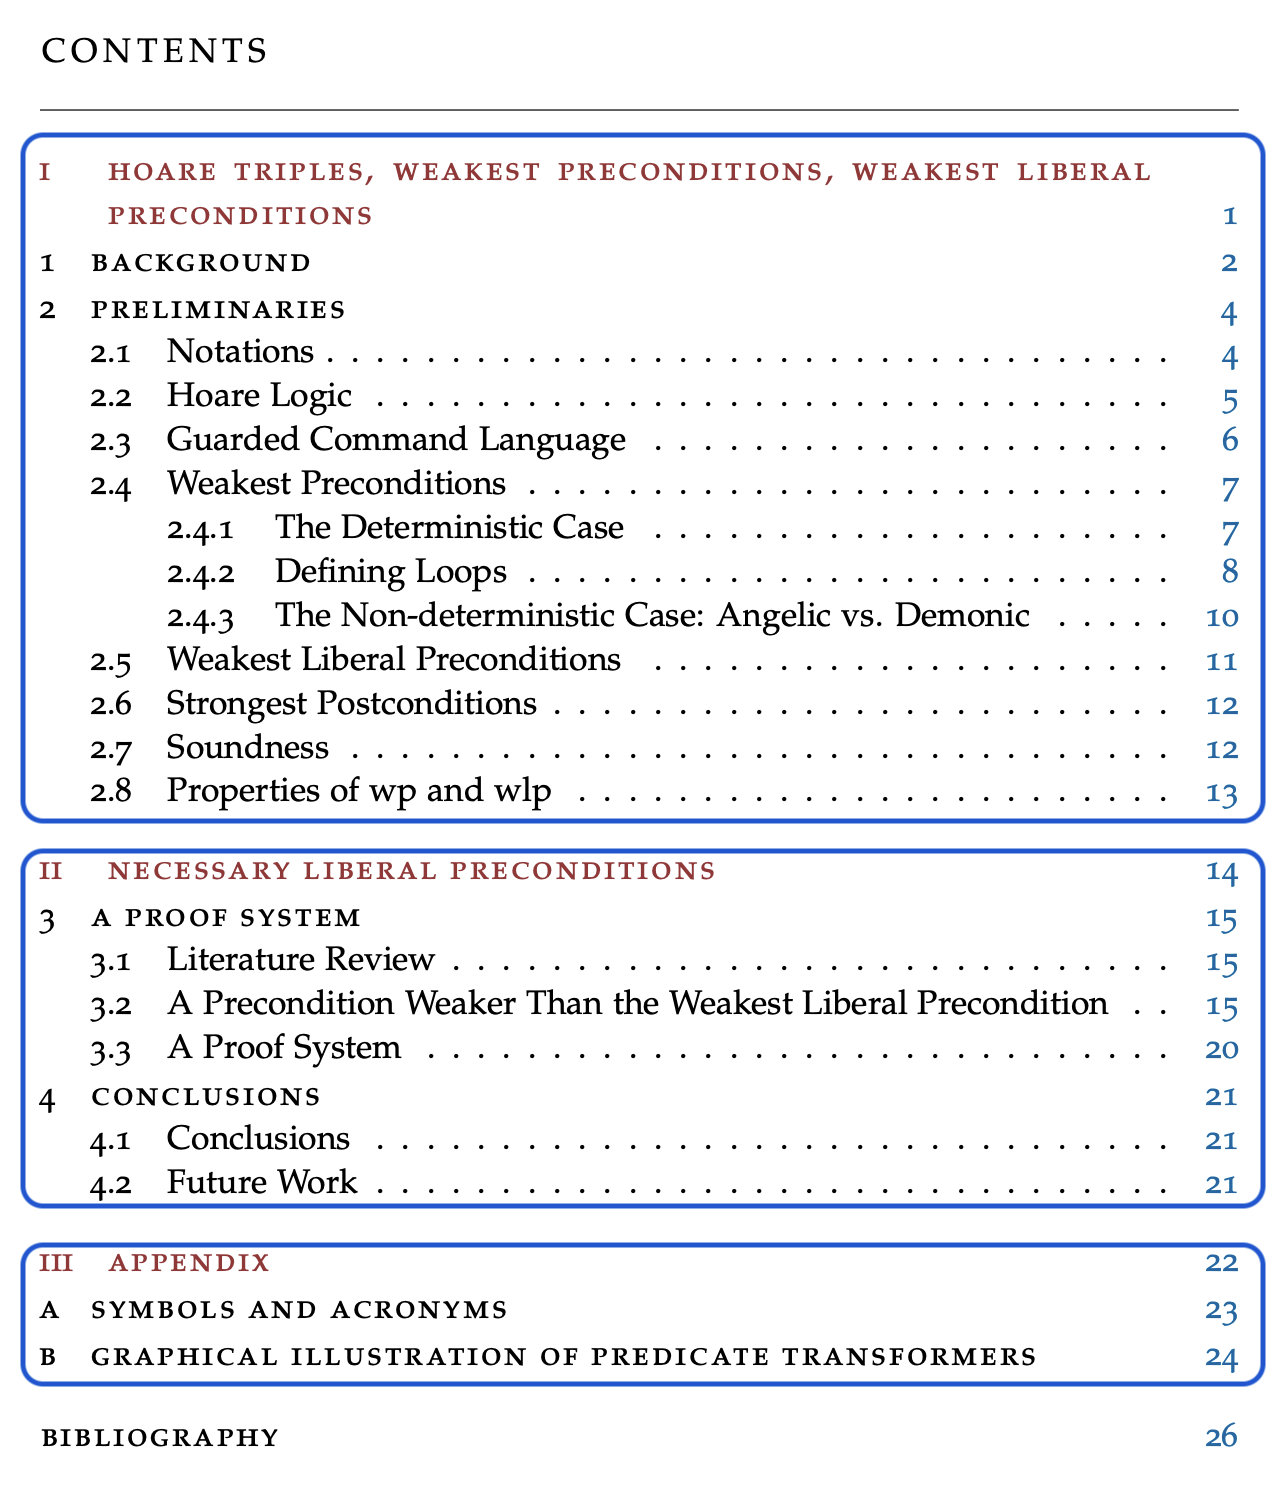
\includegraphics[width=0.75\textwidth]{images/toc-split.png} 
	  \end{figure}
	\end{minipage}
\begin{minipage}{0.49\linewidth}
	Currently divided into three parts: 
		\begin{enumerate}
		    \item[] \hl{Part I} Definitions, explanations, illustrations. 
		    \item[] \hl{Part II} Proposals, proofs, examples. 
		    \item[] \hl{Part III} Tables, figures, acronyms. 
		\end{enumerate}
	\end{minipage}
\end{frame}

% \subsection{Contents by Chapter}
\begin{frame}[fragile]
	\frametitle{Part I: Hoare Triples, Weakest Preconditions, Weakest Liberal
Preconditions}
	\begin{minipage}[t]{0.49\linewidth}	
		\begin{figure}
			\centering 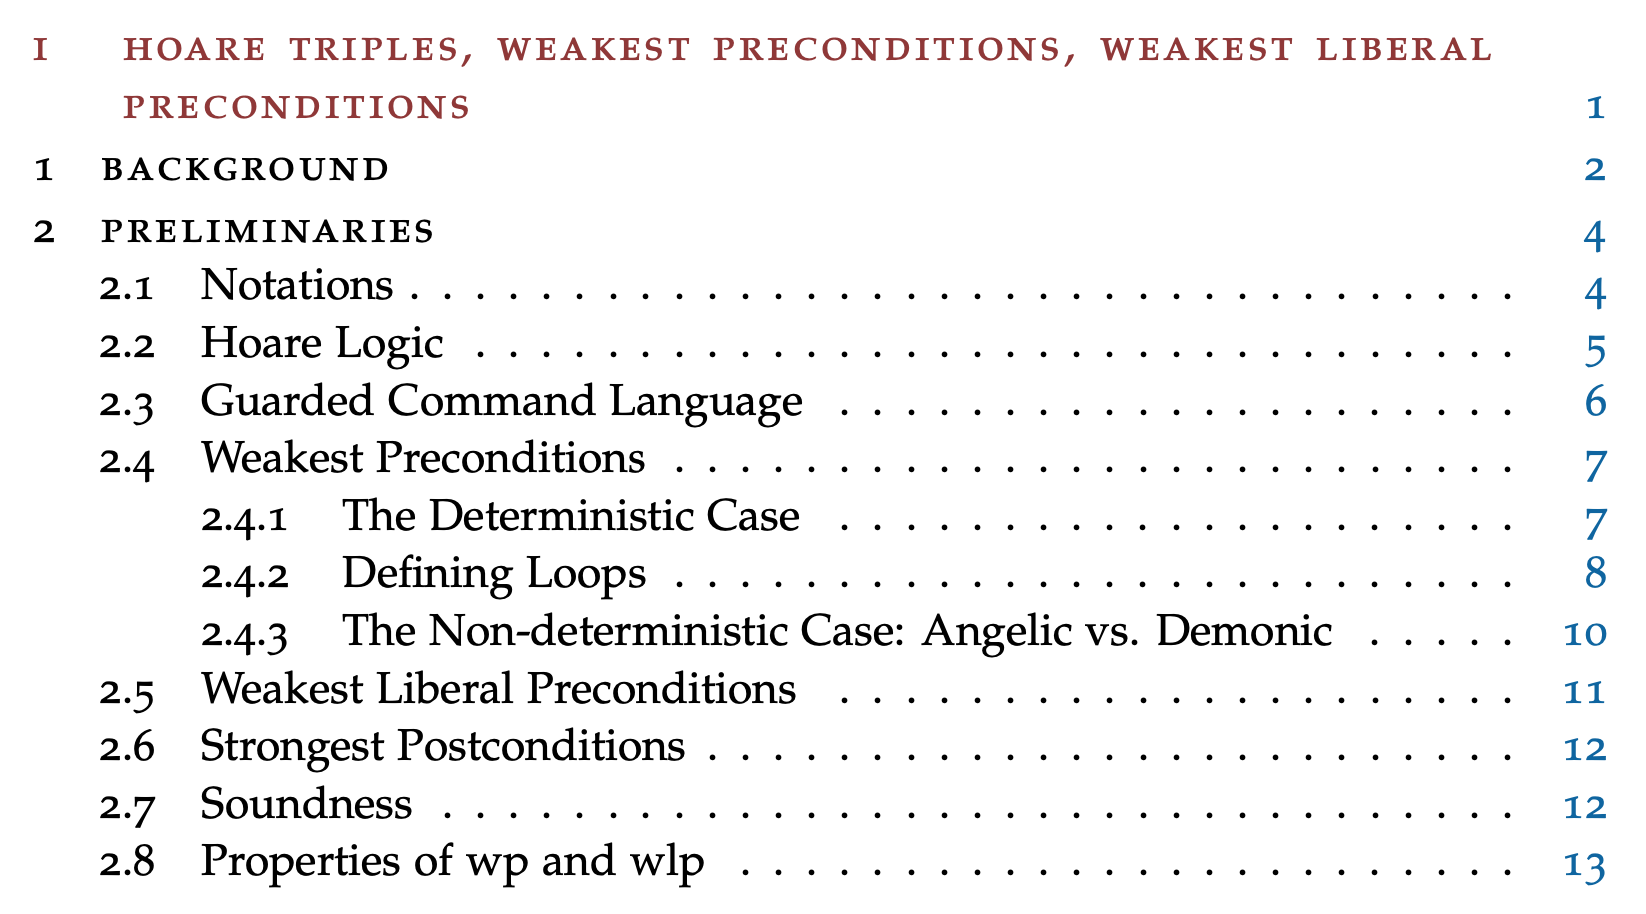
\includegraphics[width=\textwidth]{images/part1.png} 
	  \end{figure}
	\end{minipage}
	\begin{minipage}[t]{0.5\linewidth}
		\begin{enumerate}
			\item[] \hl{Chapter 1: }Background 
			\begin{itemize}
				\item Convince that proof systems are important
				\item Show the structure of the thesis
			\end{itemize}
			\item[] \hl{Chapter 2: }Preliminaries
			\begin{itemize}
				\item Table of Notations 
				\item Definitions of Hoare Triples, GCL, wp, wlp, sp
				\begin{itemize}
					\item Explain the use of lfp and gfp
				\end{itemize}
				\item Soundness: semantics of wp, wlp, sp
				\item Properties of wp and wlp that will be used in part II (forthcoming)
			\end{itemize}
		\end{enumerate}
	\end{minipage}
\end{frame}

\begin{frame}[fragile]
	\frametitle{Part II: Necessary Liberal Preconditions}
	\begin{minipage}[t]{0.49\linewidth}	
		\begin{figure}
		\centering 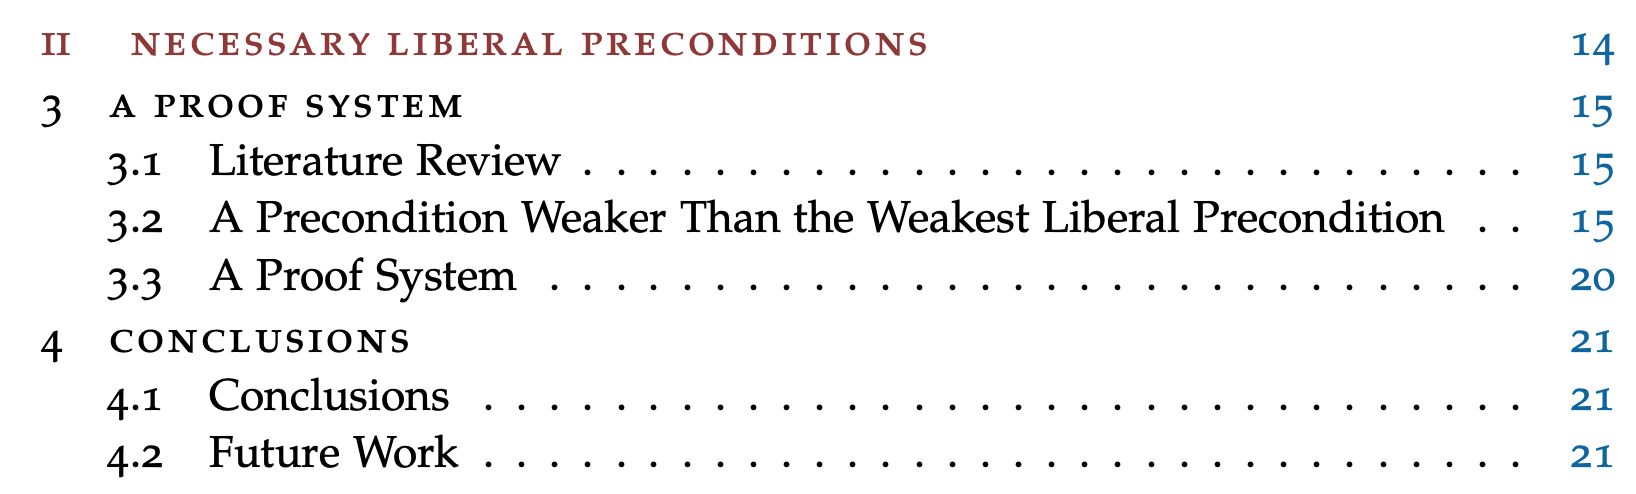
\includegraphics[width=\textwidth]{images/part2.png} 
	  \end{figure}
	\end{minipage}
	\begin{minipage}[t]{0.5\linewidth}
		\begin{enumerate}
				\item[] \hl{Chapter 3: }A Proof System
				\begin{itemize}
					\item (Forthcoming) Literature review: the similar triples that have been studied
					\item Studying a special $G$ such that $wlp.C.F \implies G$: establish wlp with angelic non-determinism using $G$ and sp. 
					\item Studying $G$ in general: proving things negatively
				\end{itemize}
			\item[] \hl{Chapter 4: }Conclusion
				\begin{itemize}
					\item Conclusion (forthcoming)
					\item Future work (forthcoming)
				\end{itemize}
	\end{enumerate}
	\end{minipage}
	
\end{frame}
\begin{frame}[fragile]
	\frametitle{Part III: Appendix}
	\begin{minipage}[t]{0.49\linewidth}	
		\begin{figure}
			\centering 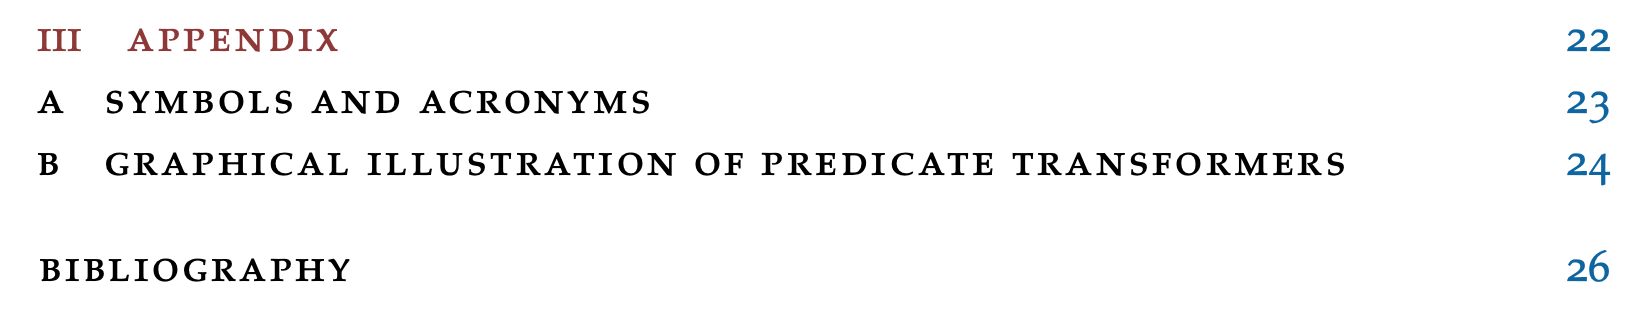
\includegraphics[width=\textwidth]{images/part3.png} 
		\end{figure}
	\end{minipage}
	\begin{minipage}[t]{0.49\linewidth}

	\end{minipage}
	
\end{frame}
\section{Contribution}
\subsection{More on images}

\begin{frame}[fragile]
	\frametitle{If you want to have multiple images, here is a template using minipage}
	\begin{itemize}
	    \item Or you can use whatever you are used to, but don't forget to include the packages! 
	    \item But using minipage, you can also easily have half image half words, or one third, or however you like.
	\end{itemize}

    \begin{minipage}{.5\textwidth}
      \centering
      
\includegraphics[width=0.7\linewidth]{images/dst.png}
    \end{minipage}%
    \begin{minipage}{.5\textwidth}
      \begin{itemize}
          \item Now there is a game that you can play!
          \begin{itemize}
              \item It is fun!
              \item You can play it with me! 
              \item Also the graphic is so cute! 
          \end{itemize}
      \end{itemize}
    \end{minipage}
\end{frame}


\section{Summary}
\subsection{}

\begin{frame}
	\frametitle{This is the summary section}
	\begin{itemize}
	    \item Intro
	    \item Body 
	    \item End
	\end{itemize}
	
	\vspace{10mm}
	\Large
	\hfill\textit{Thank you!}
\end{frame}

\begin{frame}
	\frametitle{References}
	\bibliographystyle{alpha}
	\nocite{*}
	\bibliography{literature}
\end{frame}

\end{document}